\documentclass[tikz,border=2mm]{standalone}
\usepackage[utf8]{inputenc}
\usepackage{tikz}
\usetikzlibrary{decorations.pathreplacing, positioning}

\begin{document}
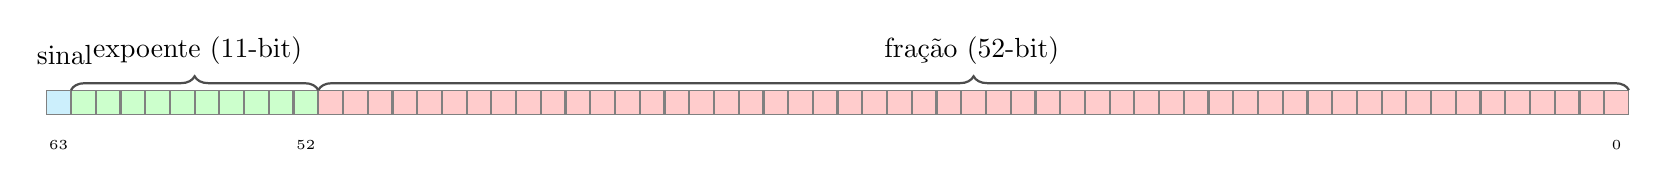
\begin{tikzpicture}[node distance=0.0cm]
    \tikzset{
        bit/.style={
            rectangle,
            draw=black!50,
            inner sep=0pt,
            minimum size=0.3cm,
            text centered,
            font=\tiny\sffamily
        }
    }

    \node[bit, fill=cyan!20] (bit63) at (0,0) {};
    \node[bit, fill=green!20, right=of bit63] (bit62) {};
    \node[bit, fill=green!20, right=of bit62] (bit61) {};
    \node[bit, fill=green!20, right=of bit61] (bit60) {};
    \node[bit, fill=green!20, right=of bit60] (bit59) {};
    \node[bit, fill=green!20, right=of bit59] (bit58) {};
    \node[bit, fill=green!20, right=of bit58] (bit57) {};
    \node[bit, fill=green!20, right=of bit57] (bit56) {};
    \node[bit, fill=green!20, right=of bit56] (bit55) {};
    \node[bit, fill=green!20, right=of bit55] (bit54) {};
    \node[bit, fill=green!20, right=of bit54] (bit53) {};

    \node[bit, fill=red!20, right=of bit53] (bit52) {};
    \node[bit, fill=red!20, right=of bit52] (bit51) {};
    \node[bit, fill=red!20, right=of bit51] (bit50) {};
    \node[bit, fill=red!20, right=of bit50] (bit49) {};
    \node[bit, fill=red!20, right=of bit49] (bit48) {};
    \node[bit, fill=red!20, right=of bit48] (bit47) {};
    \node[bit, fill=red!20, right=of bit47] (bit46) {};
    \node[bit, fill=red!20, right=of bit46] (bit45) {};
    \node[bit, fill=red!20, right=of bit45] (bit44) {};
    \node[bit, fill=red!20, right=of bit44] (bit43) {};
    \node[bit, fill=red!20, right=of bit43] (bit42) {};
    \node[bit, fill=red!20, right=of bit42] (bit41) {};
    \node[bit, fill=red!20, right=of bit41] (bit40) {};
    \node[bit, fill=red!20, right=of bit40] (bit39) {};
    \node[bit, fill=red!20, right=of bit39] (bit38) {};
    \node[bit, fill=red!20, right=of bit38] (bit37) {};
    \node[bit, fill=red!20, right=of bit37] (bit36) {};
    \node[bit, fill=red!20, right=of bit36] (bit35) {};
    \node[bit, fill=red!20, right=of bit35] (bit34) {};
    \node[bit, fill=red!20, right=of bit34] (bit33) {};
    \node[bit, fill=red!20, right=of bit33] (bit32) {};
    \node[bit, fill=red!20, right=of bit32] (bit31) {};
    \node[bit, fill=red!20, right=of bit31] (bit30) {};
    \node[bit, fill=red!20, right=of bit30] (bit29) {};
    \node[bit, fill=red!20, right=of bit29] (bit28) {};
    \node[bit, fill=red!20, right=of bit28] (bit27) {};
    \node[bit, fill=red!20, right=of bit27] (bit26) {};
    \node[bit, fill=red!20, right=of bit26] (bit25) {};
    \node[bit, fill=red!20, right=of bit25] (bit24) {};
    \node[bit, fill=red!20, right=of bit24] (bit23) {};
    \node[bit, fill=red!20, right=of bit23] (bit22) {};
    \node[bit, fill=red!20, right=of bit22] (bit21) {};
    \node[bit, fill=red!20, right=of bit21] (bit20) {};
    \node[bit, fill=red!20, right=of bit20] (bit19) {};
    \node[bit, fill=red!20, right=of bit19] (bit18) {};
    \node[bit, fill=red!20, right=of bit18] (bit17) {};
    \node[bit, fill=red!20, right=of bit17] (bit16) {};
    \node[bit, fill=red!20, right=of bit16] (bit15) {};
    \node[bit, fill=red!20, right=of bit15] (bit14) {};
    \node[bit, fill=red!20, right=of bit14] (bit13) {};
    \node[bit, fill=red!20, right=of bit13] (bit12) {};
    \node[bit, fill=red!20, right=of bit12] (bit11) {};
    \node[bit, fill=red!20, right=of bit11] (bit10) {};
    \node[bit, fill=red!20, right=of bit10] (bit9) {};
    \node[bit, fill=red!20, right=of bit9] (bit8) {};
    \node[bit, fill=red!20, right=of bit8] (bit7) {};
    \node[bit, fill=red!20, right=of bit7] (bit6) {};
    \node[bit, fill=red!20, right=of bit6] (bit5) {};
    \node[bit, fill=red!20, right=of bit5] (bit4) {};
    \node[bit, fill=red!20, right=of bit4] (bit3) {};
    \node[bit, fill=red!20, right=of bit3] (bit2) {};
    \node[bit, fill=red!20, right=of bit2] (bit1) {};
    \node[bit, fill=red!20, right=of bit1] (bit0) {};


    \node[above=2mm of bit62, anchor=south west] (exptlabel) {expoente (11-bit)};
    \node[above=2mm of bit30, anchor=south west] (fractlabel) {fração (52-bit)};
    \node[above=2mm of bit63, anchor=south west, xshift=-4mm] (signlabel) {sinal};

    \draw [decorate,decoration={brace,amplitude=5pt,raise=0pt}, thick, black!70]
    (bit62.north west) -- (bit53.north east) node [midway,above=3pt] {};

    \draw [decorate,decoration={brace,amplitude=5pt,raise=0pt}, thick, black!70]
    (bit52.north west) -- (bit0.north east) node [midway,above=3pt] {};

    \node[below=2mm of bit63] {\tiny 63};
    \node[below=2mm of bit53] {\tiny 52};
    \node[below=2mm of bit0] {\tiny 0};


\end{tikzpicture}
\end{document}
